\part{Linear baseline model}
\label{part:linear_baseline}

%------------------------------------

\section{About this part}
\label{section:LBM_about_part}
A good linear model available in the SciKit Learn library is the Logistic Regression model.
This model is often used as a linear baseline model to compare other models with.
Only models scoring better then this linear baseline model should be considered.
This part discusses the parameters found to be optimal for this model in this setting and the road to finding these optimal parameters.
The Python-based Jupyter Notebook corresponding with this part is \emph{linear\_baseline\_model.ipynb}.
This notebook will form a \emph{template} for future model exploration.

%------------------------------------

\section{Layout of the code}
\label{section:LBM_layout_of_code}

The code is split into different steps.
Each step has some explanation in a comment or refers to a section in this report. 
This makes the code easy to read.
At the end of the Jupyter Notebook, optimisation of the model is performed.
This optimisation includes all previous steps, but these are now taken care of all in once.
This is a bit more complicated, hence why the code is split into steps at the beginning of the notebook.
The optimal parameters found are used in the steps in the beginning.
This means the resulting model from the code split into steps is the optimal model.

%------------------------------------

\section{Scoring used to evaluate the model}
\label{section:LBM_scoring_used}

The multi-class Log Loss score of a validation set taken from the training set is used to evaluate a model.
This scoring strategy is the same as used in the Kaggle competition.
An important note to make is that the unbalance, as discussed in section \ref{section:DA_data_distribution}, might make this score overly dependent on classes which have many instances.
This is an open issue discussed in section \ref{section:open_issues}.


%------------------------------------

\section{Fine-tuning the input}
\label{section:LBM_finetuning_features}
The first step in finding optimal settings for the model is finding optimal settings for the input of the model.
In this case, the parameters that can control the input are the number of features each image has and the descriptor used as discussed in part \ref{part:data_analysis}.
SIFT is often referred to as the most famous and successful of the descriptor, but all of them should be explored.
In general, more features often correspond to a better score, however, including many features can lead to overfitting of the model.
The following values were tried initially:
\begin{itemize}
    \item Descriptors: DAISY, ORB, FREAK, LUCID, VGG, BoostDesc, SIFT.
    \item Feature amounts: 5, 20, 50, 100, 150, 250 and 500.
\end{itemize}

A comparison was done by averaging the multi-class Log Loss score over 5 iterations for each of these feature amounts and descriptors.
Multiple iterations are needed since these methods make use of random values.
A lower score means a better performing model.
All of the resulting scores plotted per descriptor (\emph{small} amounts) can be found in the figures list at the end of this report.
Only the test score results are of significance.
There are 2 ways of looking at this data.
The descriptor that achieves the minimum with a certain feature amount can be seen as the optimal setting.
However, since clustering is used, one can consider the \emph{elbow method} to determine the optimal setting as well.
In figure \ref{fig:2-LBM-test_scores_best_small} both of these optimum are plotted.
When taking into consideration the elbow method, the \emph{SIFT} descriptor performs best with a feature amount around 100.
When looking at the minimum, it seems that the \emph{DAISY} descriptor would come out on top with a small margin.
The SIFT approach seems more viable since the difference in score is minimal and the SIFT approach is more general and needs a lot less computation work for training.
The Daisy approach has signs of overfitting.
The difference of score between unseen test data and training data is considerably larger than was the case with the optimum of SIFT.

To validate that the DAISY descriptor would reach the absolute minimum, an additional loop was made to test larger feature amounts: 500, 750, 1000, 1250 and 1500.
All of the resulting scores plotted per descriptor (\emph{large} amounts) can be found in the figures list at the end of this report as well.
In figure \ref{fig:2-LBM-test_scores_best_large}, both of these optimum are plotted once again.
It becomes apparent that the \emph{DAISY} descriptor does indeed have the absolute minimum of all descriptors, albeit with only a small lead.
It also becomes apparent that overfitting is indeed possible by increasing the feature amount!
The optimum was found to be 1500 as can be seen in figure \ref{fig:2-LBM-feature_amount_daisy_daisy_optimal} available in the figures list.
Since the difference with the SIFT approach is negligible and this approach shows signs of overfitting, it isn't explored further.

\begin{figure}[H]
    \centering
    \fbox{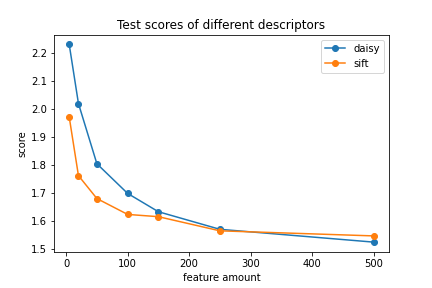
\includegraphics[width=0.7\linewidth]{images/2-LBM-test_scores_best_small.png}}
    \captionsetup{width=0.65\linewidth}
    \captionsetup{justification=centering}
    \caption{Scores in multi-class Log Loss of the Logistic Regression model using different (small) amounts of features and descriptors.}
    \label{fig:2-LBM-test_scores_best_small}
\end{figure}

\begin{figure}[H]
    \centering
    \fbox{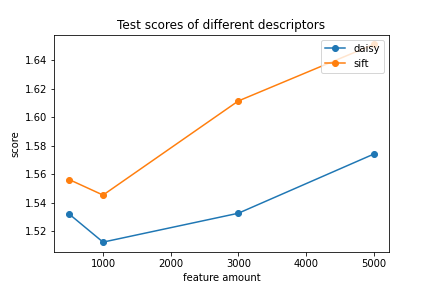
\includegraphics[width=0.7\linewidth]{images/2-LBM-test_scores_best_large.png}}
    \captionsetup{width=0.65\linewidth}
    \captionsetup{justification=centering}
    \caption{Scores in multi-class Log Loss of the Logistic Regression model using different (large) amounts of features and descriptors.}
    \label{fig:2-LBM-test_scores_best_large}
\end{figure}


%------------------------------------

\section{Fine-tuning the validation set}
\label{section:LBM_finetuning_validation_set}

Since the training data is further split into a training and validation set, this splitting can also be fine-tuned.
Later progress might even change this approach altogether, as discussed in section \ref{section:further_development}.
For now, the parameter that can be fine-tuned is \emph{test\_size} and whether or not to take into account that the data set is unbalanced.
The latter is quite obvious as discussed in section \ref{section:DA_data_distribution}.
The splitting should thus be done with the unbalance in mind since using pure random splitting could lead to validation or training sets without instances of specific classes.
When making the training set to large, overfitting becomes more likely.
When making the training set to small, the model might not be fit enough.
When making the validation set to small, the scores might not be representative enough.
A healthy balance has to be found.
Ideally, there would be enough instances in the training set to make a specific enough model and there would be enough models in the validation set to get a representative score. 
The following values were used for testing:
\begin{itemize}
    \item Descriptors: SIFT
    \item Feature amounts: 100
    \item Test sizes: 5\%, 10\%, 15\%, 20\%, 25\%, 30\%, 40\%, 50\%.
\end{itemize}

Figure \ref{fig:2-LBM-test_size_sift} shows the result of this experiment.
It is visible that with a test size of higher then 30\%, the model seems to perform worse since it doesn't have enough training data.
When taking a test size that is too small, it seems that the results aren't representative. 
A healthy balance seems to be around 15\%.
 
\begin{figure}[H]
    \centering
    \fbox{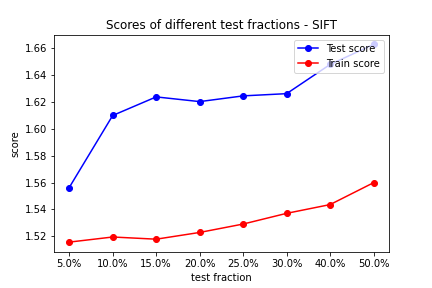
\includegraphics[width=0.7\linewidth]{images/2-LBM-test_size_sift.png}}
    \captionsetup{width=0.65\linewidth}
    \captionsetup{justification=centering}
    \caption{Scores in multi-class Log Loss of the SIFT driven Logistic Regression model using different test sizes.}
    \label{fig:2-LBM-test_size_sift}
\end{figure}



%------------------------------------

\section{Fine-tuning the model parameters}
\label{section:LBM_finetuning_model}

Now that all of the parameters available for the input are fine-tuned, the parameters of the model itself can be optimized.
As found in the documentation of the \emph{LogisticRegression} function available in the SciKit Learn library there are multiple (optional) parameters \citep{scikit_learn}.
The most interesting ones are:
\begin{itemize}
    \item \emph{solver}
    \begin{itemize}
        \item Specifies which solver should be used for the optimization problem in the model.
        \item \emph{lbfgs} is used as default and whilst a little slow, this parameter doesn't require further fine-tuning.
    \end{itemize}
    \item \emph{penalty}
    \begin{itemize}
        \item Since the \emph{lbfgs} solver is used, the default \emph{l2} penalization norm is the only one that can be used.
    \end{itemize}
    \item \emph{class\_weight}
    \begin{itemize}
        \item This parameter defaults to None but can be set to balanced to take into account the unbalance in our data, as discussed in section \ref{section:DA_data_distribution}.
        \item The results with this parameter set to balanced will be studied.
    \end{itemize}
    \item \emph{C}
    \begin{itemize}
        \item The regularisation hyperparameter C defaults to 1. Fine-tuning this could boost performance.
    \end{itemize}
    \item \emph{max\_iter}
    \begin{itemize}
        \item This parameter can be changed so that convergence might be found, which is not the case right now.
    \end{itemize}
    \item \emph{fit\_intercept}
    \begin{itemize}
        \item Boolean that specifies if a constant (a.k.a. bias or intercept) should be added to the decision function.
        \item The results with this parameter set to true and false should be checked.
    \end{itemize}
\end{itemize}


Before experimenting, it was assumed that changing the class weight parameter to balanced would enhance the performance.
This was assumed because the training data is very unbalanced whilst \emph{normal} input for model predictions wouldn't show this unbalance.
Neither using the generated validation sets shown in figure \ref{fig:2-LBM-model_weight_class}, available in the figures list, nor on the Kaggle competition page, a better score was achieved.
The fact that the performance isn't better for the validation sets isn't unexpected.
This is due to the unbalance of the training set also being apparent in the validation set since this is a subset.
However, the fact that the score is worse on the Kaggle competition, a 0.06 difference, is not expected.
Perhaps changing this parameter has more impact than was first assumed.

Setting the fit intercept parameter to false has a negative impact, albeit minor.
This is visualised in figure \ref{fig:2-LBM-model_fit_intercept} available in the figures list.
This parameter will be kept on the default, being true.

The default value for the maximum allowed iterations is 100.
With the current settings, convergence is not always reached after 100 iterations.
The following values were tried: 50, 100, 150, 200 and 250.
Since convergence is reached after 250 times in all test cases, this value is used for maximum iterations.

Finally the hyperparameter C has to be optimized.
This was done by using \emph{GridSearchCV} from the Sci Kit Learn library.
This performs an exhaustive search over specified parameter values for the model.
A similar result should be reached by performing the more manual methods used for previous parameters.
In this case the following potential C values were tried: 0.00001, 0.0001, 0.001, 0.01 , 0.1, 0.5, 1.0, 1.5, 3, 5, 10, 100, 1000, 10000
According to Grid Search, 3 is the best value for C, which happens to be close to the default of 1.
If doing the same experiment with the manual method used for the other parameters, the same can be concluded.
This manual method is visualised in figure \ref{fig:2-LBM-model_manual_c}.
This also shows the manual method is most likely just as good and offers greater insight into the working.


\begin{figure}[H]
    \centering
    \fbox{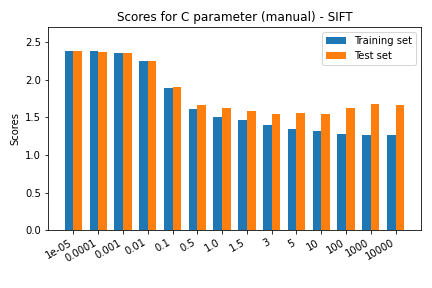
\includegraphics[width=0.7\linewidth]{images/2-LBM-model_manual_c.png}}
    \captionsetup{width=0.65\linewidth}
    \captionsetup{justification=centering}
    \caption{Scores in multi-class Log Loss of the SIFT driven Logistic Regression model using different test sizes.}
    \label{fig:2-LBM-model_manual_c}
\end{figure}


%------------------------------------

\section{The optimal settings for this model}
\label{section:LBM_optimal}

After all the fine-tuning discussed in the previous sections, an optimal model can be formed.
The optimal settings and received score for the SIFT descriptor are:
\begin{itemize}
    \item Descriptor used: SIFT
    \item Feature amounts: 100
    \item Sample size: 15\%
    \item Class weight: None
    \item C: 3
    \item Max it-er: 250
    \item Fit intercept: false
    \item Score received from validation set: 1.48756
    \item Score received on Kaggle: 1.60289
\end{itemize}

